\section{Conclus{\~a}o}
\label{sec:conclusao}
Com uma determinada padroniza{\c c}{\~a}o do modelo de branching e versionamento de projetos, {\'e} tend{\^e}ncia diminuir a ocorr{\^e}ncia dos problemas do inferno de depend{\^e}ncias (dependency hell) do projeto. No atual presente da escrita deste artigo, tal modelo ainda n{\~a}o foi testado, n{\~a}o sendo poss{\'i}vel comprovar a sua efic{\'a}cia. Uma vis{\~a}o geral do modelo pode ser visto na figura \ref{fig:branching}.

\begin{figure}[h!]
	\centering
	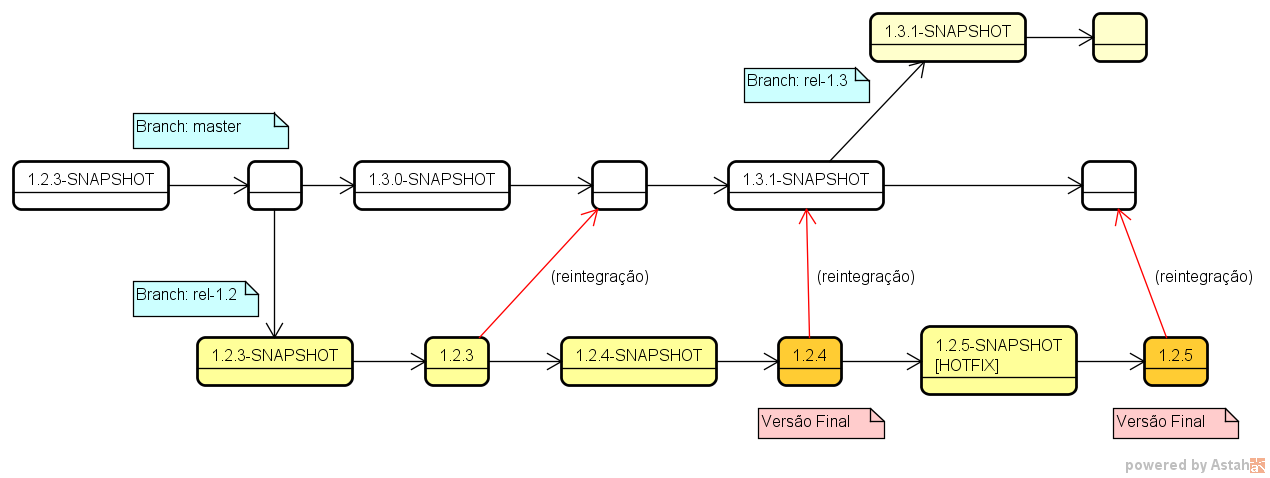
\includegraphics[width=1\linewidth]{img/branching_otojr}
	\caption[Modelo de branching]{Modelo de branching porposto}
	\label{fig:branching}
\end{figure}